\documentclass[11pt,a4paper]{article}

\usepackage[T1]{fontenc}
\usepackage{lmodern}
\usepackage[margin=2.3cm]{geometry}
\usepackage{graphicx}
\usepackage{booktabs}
\usepackage{amsmath}
\usepackage{xcolor}
\usepackage{enumitem}
\usepackage[hidelinks]{hyperref}
\usepackage{parskip}
\usepackage{tabularx}

\setlist{itemsep=2pt, topsep=4pt}
\newcommand{\strength}[1]{\par\noindent\textbf{How sure we are:} #1\par}
\newcommand{\claim}[1]{\par\smallskip\noindent\colorbox{black!6}{\parbox{\dimexpr\linewidth-2\fboxsep}{\textbf{Claim.} #1}}\par\smallskip}

\title{Findings Beyond the Headline\\[4pt] \large What the Imvo results show that the research question did not ask}
\author{NLP Project 2 group (Lily de Melo, Tawananyasha Kadango, Sally Mohlakola)}
\date{21 October 2026 --- provisional run (LaBSE pair threshold 0.55, no hand labels yet)}

\begin{document}
\maketitle

\section*{Purpose}
The paper answers two questions: do \emph{Imvo}'s isiXhosa and English sections differ in content (H1), and
does modernising the spelling change that answer (H2)? This document collects what else the results
show. Each finding states a claim, the evidence for it, why it matters, and how sure we are. Where the
evidence is weaker, we say so and name the check that would settle it.

All numbers come from \texttt{results/}. The four post-hoc checks (Findings 2, 3 and 6) are in
\texttt{src/posthoc\_checks.py} (output: \texttt{results/posthoc\_checks.txt}), and the figures here from
\texttt{docs/make\_findings\_figures.py}. Those checks reuse the trained classifiers' test predictions; nothing
was retrained. Confidence intervals (CIs) are 95\% bootstrap intervals over test issues unless stated.

\begin{table}[h]
\centering\small
\begin{tabularx}{\linewidth}{@{}clX@{}}
\toprule
& Finding & Evidence \\
\midrule
1 & Spelling modernisation changes the instrument, not the content & strong for LaBSE, partial for E5 \\
2 & The content gap of 0.196 is a lower bound & good (one post-hoc check) \\
3 & The gap is not page layout (tables, price lists) & strong \\
4 & Mean-centring with a linear probe hides real differences & strong \\
5 & Encoder geometry decides which probe works & good \\
6 & Rising separability over the decade is language, not content & good (LaBSE) \\
7 & Analysing only the English half studies a different newspaper & strong \\
8 & ``Cleaning'' rewrites names of peoples, places and God & strong (counts) \\
9 & Prefix joining adds little for the encoder & moderate (ablation only) \\
\bottomrule
\end{tabularx}
\end{table}

%-------------------------------------------------------------------------------------------------
\section{Modernisation changes the instrument, not the content}
\claim{Modernising the spelling barely changes how well the classifier tells the sections apart. It
changes how well the encoder lines the two languages up, and the measured gap moves because of that.}

\textbf{Evidence (LaBSE).}
\begin{itemize}
  \item Accuracy on all chunks: 0.786 (raw) $\to$ 0.784 (modern); change $-0.002$, CI $-0.007$ to $+0.004$.
  \item Floor (translated pairs): 0.590 $\to$ 0.571; change $-0.019$, CI $-0.043$ to $+0.005$.
  \item Since the gap is all minus floor, the gap rises by $+0.018$, and this rise is the floor's fall.
  \item Mean similarity of the reference pairs rises by $+0.005$ (CI $+0.003$ to $+0.007$). This is
  conservative: the pairs were chosen as mutual nearest neighbours in \emph{raw} space, which favours raw.
  \item More translation pairs are found above the threshold: 1{,}984 (raw), 2{,}155 (modern, $+8.6\%$),
  2{,}118 (aspiration only), 2{,}032 (prefix only).
\end{itemize}

\begin{figure}[h]
  \centering
  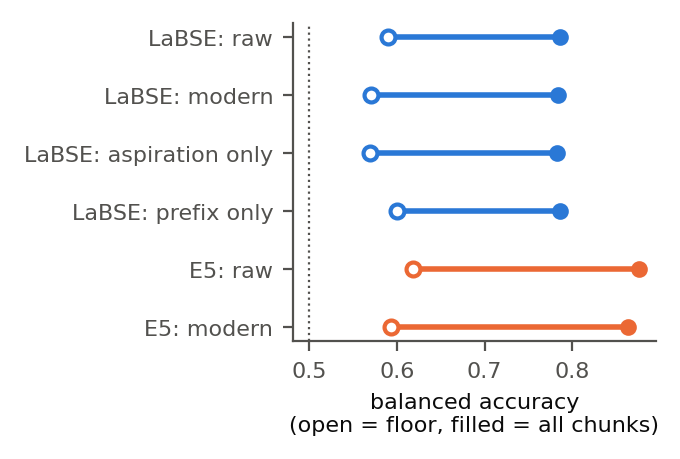
\includegraphics[width=0.55\linewidth]{figures/fig_modernisation_mechanism.png}
  \caption{For each spelling variant, the floor (open) and accuracy on all chunks (filled); the line is
  the gap. Modernising moves the open circles, not the filled ones.}
\end{figure}

\textbf{E5 is only partly consistent.} Its floor also falls ($-0.025$), but accuracy on all chunks falls
too ($-0.013$, CI $-0.019$ to $-0.007$), and pair similarity does not change ($-0.0002$). Pairs found rise
only 1.8\%. A plausible reason: LaBSE was trained specifically to match translations, so better spelling
helps it align; E5 was not, so its alignment is less sensitive to spelling.

\textbf{Why it matters.} It says \emph{which} analyses should worry about spelling. Methods that depend on
aligning the languages (finding translations, cross-lingual retrieval, removing language with pairs) are
sensitive to it. A content classifier on its own is not. Recommending ``normalise for alignment tasks''
is more useful than ``preprocessing matters''.

\strength{strong for LaBSE (the all-chunk change is tightly bounded around zero and the similarity rise
excludes zero). The floor's fall by itself is not significant; the claim rests on the all-chunk
stability. Partial for E5.}

%-------------------------------------------------------------------------------------------------
\section{The content gap is a lower bound}
\claim{Much of the floor (0.590) is not leftover language but loose or wrong ``translations''. Because
the floor is subtracted, the reported gap of 0.196 underestimates the true content difference.}

\textbf{Evidence.}
\begin{itemize}
  \item Removing one language direction drops the floor from 0.97 to 0.59; removing up to 64 more barely
  moves it (lowest 0.567). A signal that more directions cannot remove behaves unlike a language direction.
  \item Grouping the 311 test pairs into quarters by similarity (Figure~\ref{fig:floor}): the least
  similar half has floors of 0.628 and 0.647; the most similar half 0.545 and 0.538, with CIs that
  include chance. E5 shows the same trend (0.690 $\to$ 0.550).
  \item Measured against the most similar half of pairs only, the gap is \textbf{0.244} (CI 0.207 to
  0.283) for LaBSE and 0.291 (0.224 to 0.354) for E5, against 0.196 and 0.258 with all pairs.
  \item The synthetic test predicted this. With a planted gap whose clean-pair value is 0.099, adding
  40\% false pairs lowers the gap even for an oracle that sees content only (0.059, because the false
  pairs raise its floor), and the pair method finds 0.045. Noisy pairs push the estimate down, never up.
\end{itemize}

\begin{figure}[h]
  \centering
  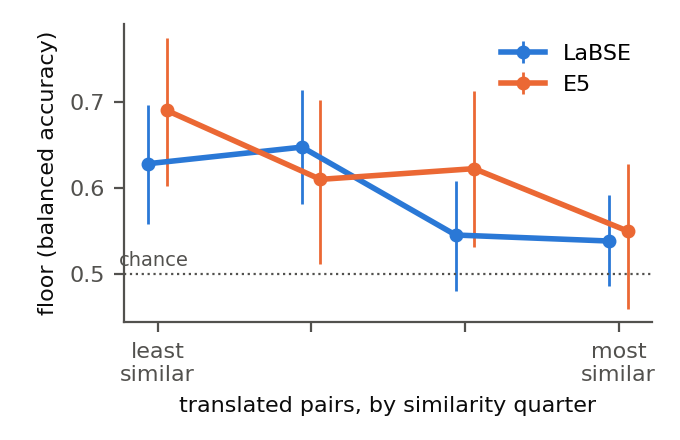
\includegraphics[width=0.5\linewidth]{figures/fig_floor_by_similarity.png}
  \caption{Floor by pair-similarity quarter (95\% CIs). The closer a pair is to a true translation, the
  closer the classifier is to guessing.}
  \label{fig:floor}
\end{figure}

\textbf{It also explains an anomaly.} The robustness run with stricter pairs ($\geq$0.65) had a
\emph{higher} floor (0.725). That run re-estimated the 64 language directions from only 362 training pairs.
Here the directions are the same and only the evaluation pairs change, and the floor falls. So the
anomaly comes from estimating the directions from too few pairs, not from stricter pairs being worse.

\textbf{Why it matters.} We can claim ``at least about 0.2'' instead of ``about 0.2'', and the main
weakness of the method (imperfect pairs) biases it towards caution.

\strength{good. The quarter grouping was chosen after seeing the main results, and very similar pairs
may also be shorter or more formulaic. Hand-labelled pairs will test this directly: true translations
should give a floor near 0.5.}

%-------------------------------------------------------------------------------------------------
\section{The gap is not page layout}
\claim{The difference between the sections is not caused by tables, price lists and other number-heavy
material that looks different to the encoder.}

\textbf{Evidence.} We removed chunks that look like tables, then chunks in which at least 30\%, 20\%,
10\% and finally 5\% of words contain a digit (Figure~\ref{fig:numbers}). At the strictest cut,
21.8\% of isiXhosa chunks and 3.0\% of English chunks are gone. The LaBSE gap moves from 0.196 to 0.185
(CI 0.155 to 0.216); the E5 gap from 0.258 to 0.265.

\begin{figure}[h]
  \centering
  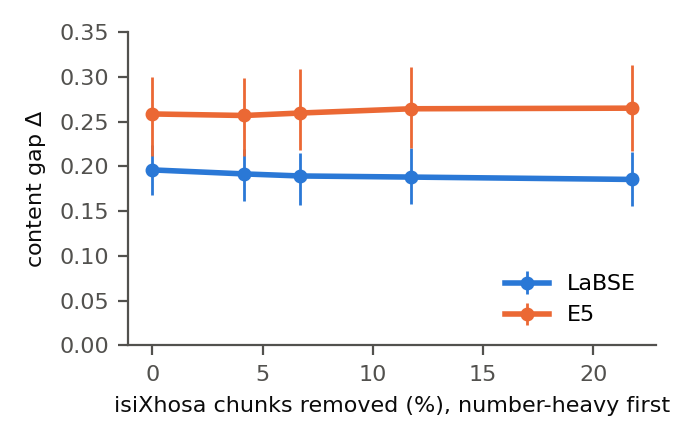
\includegraphics[width=0.5\linewidth]{figures/fig_gap_without_numbers.png}
  \caption{The gap as number-heavy chunks are removed (95\% CIs): flat.}
  \label{fig:numbers}
\end{figure}

\textbf{This corrects our own first reading.} The topic clusters most specific to isiXhosa are price
lists, land notices and sport results, and it was tempting to say those \emph{are} the difference. They are
its most extreme examples, but the gap survives without them: the difference runs through ordinary
prose as well.

\strength{strong. One limit: the classifier was trained with these chunks included; we removed them
only when evaluating.}

%-------------------------------------------------------------------------------------------------
\section{Mean-centring with a linear probe hides real differences}
\claim{The common way to remove language (subtract each language's average vector) combined with the
common way to test for differences (a linear classifier) cannot find a content difference, even when
one exists.}

\textbf{Evidence.}
\begin{itemize}
  \item Why: after mean-centring, both sections have the same average vector, so a linear classifier has
  almost nothing left to separate them by.
  \item Synthetic data with a planted difference: mean-centring reports 0.000 at every size of
  difference, while the true gap reaches 0.099.
  \item Real data: the linear probe after mean-centring scores exactly 0.500 (chance) on everything.
  \item Yet a $k$-nearest-neighbour probe on the same mean-centred vectors finds a gap of 0.065 for LaBSE
  (all 0.933, floor 0.868). The difference is still there; the linear probe cannot see it.
\end{itemize}

\textbf{Why it matters.} A study that removes language by mean-centring and reports ``no difference''
from a linear probe may be reporting an artefact. The removal method and the probe must be chosen
together. This adds to the widely used mean-centring approach rather than just reusing it.

\strength{strong for the linear case (it follows from the construction, and both data sets show it). The
kNN number has no CI and sits above a high floor; E5's kNN gap after mean-centring is only 0.022.}

%-------------------------------------------------------------------------------------------------
\section{Encoder geometry decides which probe works}
\claim{The two encoders store the same information differently, and that changes which classifier can
find it.}

\textbf{Evidence.}
\begin{itemize}
  \item E5's pair similarities are squeezed into a narrow band (median 0.847; 90\% between 0.83
  and 0.88), against a median of 0.493 for LaBSE. Its vectors point in nearly the same direction.
  \item Language sits in one direction for E5 (the floor target is reached at $k{=}1$, validation floor
  0.543) but never fully goes for LaBSE.
  \item After removing language, E5's linear probe finds a gap of 0.258 but its kNN probe only 0.046.
  For LaBSE the two agree more closely (0.196 vs 0.149).
\end{itemize}
In a space where all vectors are close together, nearest-neighbour search is dominated by what they
share, so a probe based on neighbours misses a difference that lies along one direction.

\textbf{Why it matters.} A single probe on a single encoder can mislead in either direction. It justifies
the two-encoder, two-probe design, and it is a warning for anyone who uses cosine neighbours on E5-style
embeddings.

\strength{good for the observations; the geometric explanation is the most likely one but we did not test
it directly (for example by whitening E5's vectors and rerunning kNN).}

%-------------------------------------------------------------------------------------------------
\section{Rising separability over the decade is language, not content}
\claim{The sections become easier to tell apart between 1884 and 1894, but the floor rises just as much,
so the content gap itself does not grow. Without the floor this would have looked like a historical
finding.}

\textbf{Evidence.} Accuracy on all test chunks rises from about 0.74--0.76 (1885--87) to about 0.81
(1891--94) for LaBSE: a trend of $+0.059$ per decade (CI $+0.018$ to $+0.101$); E5 agrees ($+0.052$, CI
$+0.029$ to $+0.071$). See Figure~\ref{fig:year}. Yearly floors rest on too few pairs, so we split the test
issues into two periods, each with its own floor:

\begin{center}\small
\begin{tabular}{@{}lccccc@{}}
\toprule
LaBSE & Test issues & Pair chunks & All & Floor & Gap (95\% CI) \\
\midrule
1884--89 & 40 & 412 & 0.766 & 0.573 & 0.193 (0.159 to 0.222) \\
1890--94 & 37 & 210 & 0.805 & 0.624 & 0.181 (0.133 to 0.231) \\
\bottomrule
\end{tabular}
\end{center}

The change in the gap is $-0.012$ (CI $-0.073$ to $+0.048$): the extra separability in the later period is
matched by a higher floor, i.e.\ more language signal left over, not more different content. E5 is
inconclusive ($+0.061$, CI $-0.029$ to $+0.142$).

\begin{figure}[h]
  \centering
  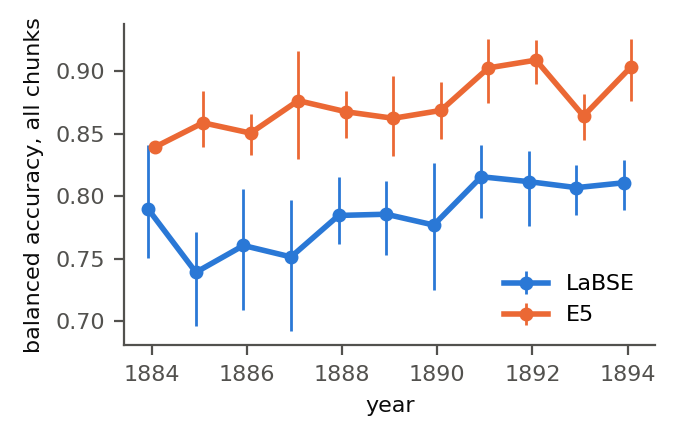
\includegraphics[width=0.5\linewidth]{figures/fig_by_year.png}
  \caption{Accuracy on all test chunks by year (95\% CIs over that year's test issues). The rise is
  matched by a rising floor (table above).}
  \label{fig:year}
\end{figure}

\textbf{Why it matters.} It is a direct demonstration of why the floor is needed: an analysis that
reported accuracy alone would have claimed that \emph{Imvo}'s two audiences drifted apart. Why the
floor rises is open; changes in print or OCR quality, or in spelling, are candidates.

\strength{good for ``no growth in the content gap'' with LaBSE (the floor is measured per period); the
periods' intervals are wide, so a small change cannot be ruled out.}

%-------------------------------------------------------------------------------------------------
\section{Analysing only the English half studies a different newspaper}
\claim{Researchers often work with the English half of bilingual sources because the tools work better
on it. For \emph{Imvo}, that would not give a smaller sample of the same paper but a different paper.}

\textbf{Evidence.}
\begin{itemize}
  \item The section difference is large (gap 0.196) and spread through ordinary prose (Finding 3), so it is
  not confined to a few genres.
  \item Whole categories are missing in English: a cluster of 1{,}211 market-price chunks contains no
  English chunk at all; land-sale notices are 95\% isiXhosa.
  \item Within an issue, the two halves' topic mixes differ twice as much as shuffled halves would
  (Jensen--Shannon divergence 0.141 vs 0.067; 91\% of test issues above their shuffled range; E5: 0.206
  vs 0.041, 100\%).
  \item The tools do favour English: LaBSE needs 2.11 subword tokens per isiXhosa word against 1.26 for
  English (67\% more). Modern isiXhosa needs 2.18, so the cost comes from the language, not the period.
\end{itemize}

\textbf{Why it matters.} It turns a general worry (English-centric tools) into a measured case: which
material gets studied is decided by tool convenience, and here that would drop the content written for
African readers.

\strength{strong for the existence and size of the difference. The topic clusters are only weakly
separated (silhouette 0.008), so they describe the difference rather than count it exactly.}

%-------------------------------------------------------------------------------------------------
\section{``Cleaning'' rewrites names of peoples, places and God}
\claim{The normaliser's changes include, systematically, the most culturally loaded words in the text.}

\textbf{Evidence.} Aspiration restoration rewrites 191 word types that the authors capitalised in at
least 90\% of their non-headline uses, 19{,}917 occurrences in all. Most are names: \emph{Xosa}$\to$\emph{Xhosa}
(587 occurrences), \emph{Tembu}$\to$\emph{Thembu} (785), \emph{Mtata}$\to$\emph{Mthatha} (559) and
\emph{Tixo}$\to$\emph{Thixo} (God; 1{,}448). Some are institutions or headings the authors capitalised,
such as \emph{Rulumente} (government). Uses in ALL CAPS are left out of the 90\% share: counting them
as lower case had hidden \emph{Tixo}, which is often set in headlines. The archive deliberately did not spell-check
the text, because the spelling of the period differs from today's.

\textbf{Why it matters.} The modern spellings are correct, but they overwrite how the writers spelled
their own people, places and God. Combined with Finding 1, the trade-off is concrete: modernising helps
LaBSE align the languages a little ($+8.6\%$ pairs), and the price is rewriting thousands of names. A
\emph{names kept} variant (both rules, likely names left as written) is in the pipeline to test whether
the gain survives without that price; it needs one more Colab run.

\strength{strong for the counts. We have not shown that names are rewritten \emph{more often} than other
words, only that they are rewritten in large numbers.}

%-------------------------------------------------------------------------------------------------
\section{Prefix joining adds little for the encoder}
\claim{Of the two modernisation rules, only restoring aspiration changes what the encoder does; joining
prefixes, although it moves the text towards the modern written standard, has no measurable effect.}

\textbf{Evidence.} Of the two rules, aspiration does all the work: it raises the gap by $+0.017$, finds
6.8\% more pairs and raises pair similarity by 0.003. Prefix joining changes the gap by $-0.009$ (CI
$-0.028$ to $+0.010$), finds only 2.4\% more pairs and leaves similarity almost unchanged ($+0.0009$). With the current normaliser,
prefix-joined text has slightly more words missing from the modern word list than raw text (31.9\% vs
31.5\%) and about the same subword tokens per word (2.117 vs 2.113). The rise is a counting effect, not
harm: the 48{,}314 joins reduce out-of-vocabulary tokens (9{,}212 to 8{,}711), but each also merges a
prefix that is always in the list (\emph{e}, \emph{ku}, \emph{kwe}) into its word, removing 48{,}314 known
tokens from the count. Most joins attach a prefix to a place name (\emph{e Qonce}$\to$\emph{eQonce},
\emph{kwe Nciba}$\to$\emph{kweNciba}), whose stem keeps its 1880s spelling.

\textbf{Why it matters.} Moving towards the prescriptive standard is not automatically moving towards
what the encoder learned from; a normaliser built for NLP should be judged by its effect on the encoder.

\strength{moderate for ``adds little'' (its change in the gap is small and its interval includes zero). Why
it adds little is not tested directly; the tokenisation numbers show joining barely changes how the
encoder segments the text.}

%-------------------------------------------------------------------------------------------------
\section*{What these findings do \emph{not} show}
\begin{itemize}
  \item \textbf{Editorial intent.} We measure what was printed, not why.
  \item \textbf{That modernisation is harmless or harmful.} H2 is formally inconclusive: the change in the
  gap ($+0.018$, 90\% CI $-0.003$ to $+0.037$) is neither within our $\pm$0.02 margin nor clearly
  different from zero.
  \item \textbf{Final numbers.} Every result uses the provisional pair threshold of 0.55; hand-labelled pairs
  will change the numbers somewhat. Finding 2 is the most likely to sharpen.
\end{itemize}

\end{document}
